
\documentclass{article}

%-------------------------------------------------------------------------------------------------------------
%  package
%--------------------------------------------------------------------------------------------------------------
%版面規劃(a4大小,上下左右距0.9inch)
\usepackage[a4paper,margin=0.9in]{geometry}
%和插入圖片相關的package
\usepackage{graphicx}
\usepackage[FIGTOPCAP]{subfigure}
\usepackage{amsmath,booktabs,threeparttable,url, bm}
%\usepackage[hyphenbreaks]{breakurl}
%連結註腳網頁
\usepackage[colorlinks,linkcolor=blue]{hyperref}
%中文化package
\usepackage{CJKutf8}

%\newcommand{\cntext}{\begin{CJK}{UTF8}{bsmi}\end{CJK}}

\title{Assignment 4 of Computational Astrophysics in NTHU}
\author{Wei-Hsiang Yu 游惟翔}


%-------------------------------------------------------------------------------------------------------------
%  文件開始
%--------------------------------------------------------------------------------------------------------------
\begin{document}

\begin{CJK}{UTF8}{bsmi}
%中文化需要加上此行才有title/author/date
\maketitle
\end{CJK}


%-------------------------------------------------------------------------------------------------------------
%  Written Assignments
%--------------------------------------------------------------------------------------------------------------
\section{Written Assignments}
\underline{\textbf{Q1 : Vector Norms.}}\\

For the vector x
$x=
{\begin{bmatrix}
-1.6,& 1.2
\end{bmatrix}}^T
$
From the lecture we know that:
\[ 
First\ norm:{||x||}_1=\sum_{i=1}^{n}|x_i|
\qquad \mbox{(sum of each element)=2.8}
\]
\[ 
Second\ norm:{||x||}_2=(\sum_{i=1}^{n}|x_i|^2)^{\frac{1}{2}}
\qquad \mbox{(square root the sum of each element does square)=2}
\]
\[ 
Infinity\ norm:{||x||}_\infty=\max_{1 \leq i \leq n}|x_i|
\qquad \mbox{(maximum element)=1.6}
\]
\underline{\textbf{Q2 : Matrix Norms.}}\\

For the matrix A
\[
A=
{\begin{bmatrix}
7 & -3 & 2\\
1 & 1 & 5\\
2 &-2 & 1
\end{bmatrix}}
\]

From the lecture we know that:
\[ 
First\ norm:{||A||}_1=\max_{j}\sum_{i=1}^{n}|a_{ij}|
\qquad \mbox{(the maximum absolute \textbf{column} sum)=10}
\]
\[ 
Infinity\ norm:{||A||}_\infty=\max_{i}\sum_{j=1}^{n}|a_{ij}|
\qquad \mbox{(the maximum absolute \textbf{row} sum)=12}
\]
\underline{\textbf{Q3 : Matrix calculation.}}\\
\[
Ax=
{\begin{bmatrix}
1 & 2 & 2\\
4 & 6 & 8\\
4 & 8 & 10
\end{bmatrix}}
{\begin{bmatrix}
x_1\\
x_2\\
x_3
\end{bmatrix}}
=
{\begin{bmatrix}
4\\
6\\
10
\end{bmatrix}}
=b
\]
\textbf{3a. Gaussian elimination}\\

Eliminate matrix A, we can use $4\times first\ row$ to subtract the $third\ row$(step1), and also subtract the $second\ row$ by $4\times first\ row$ (step2).
\[
{\begin{bmatrix}
1 & 2 & 2\\
4 & 6 & 8\\
4 & 8 & 10
\end{bmatrix}}
\Rightarrow
{\begin{bmatrix}
1 & 2 & 2\\
4 & 6 & 8\\
0 & 0 & 2
\end{bmatrix}}_{step1}
\Rightarrow
{\begin{bmatrix}
1 & 2 & 2\\
0 &-2 & 0\\
0 & 0 & 2
\end{bmatrix}}_{step2}
=U
\]

Finally, we can solve this equation.
\[
{\begin{bmatrix}
1 & 2 & 2\\
0 &-2 & 0\\
0 & 0 & 2
\end{bmatrix}}
{\begin{bmatrix}
x_1\\
x_2\\
x_3
\end{bmatrix}}
=
{\begin{bmatrix}
4\\
6\\
10
\end{bmatrix}}
\quad
\Rightarrow
\quad
{\begin{bmatrix}
x_1\\
x_2\\
x_3
\end{bmatrix}}
=
{\begin{bmatrix}
0\\
-3\\
5
\end{bmatrix}}
\]
\textbf{3b.\&3c. LU factorization}\\

See 3a. we have already gotten the Upper triangular matrix U. The lower triangular matrix L is described by the steps in 3a.(The subtracted steps using the first row can be viewed as improving of the unit matrix I, but opposite sign)
And we also see the lecture that $A=LU$
So we finally get the LU factorization:
\[
A=
{\begin{bmatrix}
1 & 2 & 2\\
4 & 6 & 8\\
4 & 8 & 10
\end{bmatrix}}
=LU
=
{\begin{bmatrix}
1 & 0 & 0\\
4 & 1 & 0\\
4 & 0 & 1
\end{bmatrix}}
{\begin{bmatrix}
1 & 2 & 2\\
0 &-2 & 0\\
0 & 0 & 2
\end{bmatrix}}
\]
\underline{\textbf{Q4 : Cholesky factorization.}}\\
\[
{\begin{bmatrix}
4 &-1 &-1\\
-1& 4 &-1\\
-1&-1 & 4
\end{bmatrix}}
\]
Cholesky factorization has the feature that it can decompose a matrix into two triangular matrix L \& U, which are transpose to each other($U=L^T$)
Let's derive the solution of doing Cholesky factorization
\footnote{Cholesky factorization:\href{https://ccjou.wordpress.com/2010/09/16/cholesky-\%E5\%88\%86\%E8\%A7\%A3/}{https://ccjou.wordpress.com/2010/09/16/cholesky-\%E5\%88\%86\%E8\%A7\%A3/}}:


\[
A=
{\begin{bmatrix}
a_{11} & a_{12} & a_{13}\\
a_{21} & a_{22} & a_{23}\\
a_{31} & a_{32} & a_{33}
\end{bmatrix}}
=
GG^T
=
{\begin{bmatrix}
g_{11} & 0 & 0\\
g_{21} & g_{22} & g\\
g_{31} & g_{32} & g_{33}
\end{bmatrix}}
{\begin{bmatrix}
g_{11} & g_{12} & g_{13}\\
0 & g_{22} & g_{23}\\
0 & 0 & g_{33}
\end{bmatrix}}
\]
\[
=
{\begin{bmatrix}
g^2_{11} & g_{21}g_{11} & g_{31}g_{11}\\
g_{21}g_{11} & g^2_{21}+g^2_{22} & g_{31}g_{21}+g_{32}g_{22}\\
g_{31}g_{11} & g_{31}g_{21}+g_{32}g_{22} & g^2_{11}+g^2_{22}+g^2_{33}
\end{bmatrix}}
\]

So, we can use this solution to find out the Cholesky factorization of the problem:
\[
{\begin{bmatrix}
4 &-1 &-1\\
-1& 4 &-1\\
-1&-1 & 4
\end{bmatrix}}
=
{\begin{bmatrix}
2 & 0 & 0\\
-\frac{1}{2}& \frac{\sqrt{15}}{2} & 0\\
-\frac{1}{2}& -\frac{5}{2\sqrt{15}} & \sqrt{\frac{10}{3}}
\end{bmatrix}}
{\begin{bmatrix}
2 & -\frac{1}{2} & -\frac{1}{2}\\
0& \frac{\sqrt{15}}{2} &-\frac{5}{2\sqrt{15}}\\
0&0 & \sqrt{\frac{10}{3}}
\end{bmatrix}}
\]




%-------------------------------------------------------------------------------------------------------------
%  Programming Assignments
%--------------------------------------------------------------------------------------------------------------
\section{Programming Assignments}
%Q2---------------------------------------------------------------------
\underline{\textbf{Q1 : Error of solving the system.\\}}\\
\[
{\begin{bmatrix}
1 & 1+\epsilon\\
1-\epsilon& 1
\end{bmatrix}}
{\begin{bmatrix}
x_1\\
x_2
\end{bmatrix}}
=
{\begin{bmatrix}
1+\epsilon+\epsilon^2\\
1
\end{bmatrix}}
\]
% %-------------------------------
\begin{figure}[h]
    \centering
    \subfigure[error when $\epsilon=1e-11$ ]{
        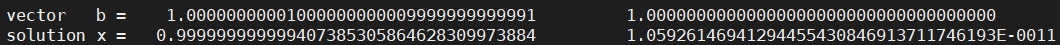
\includegraphics[scale=0.5]{pro1-11.jpg}
        \label{fig1_11}
    }
    \subfigure[error when $\epsilon=1e-12$]{
        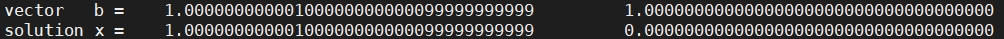
\includegraphics[scale=0.5]{pro1-12.jpg}
        \label{fig1_12} 
    }
    \subfigure[error when $\epsilon=1e-6$]{
        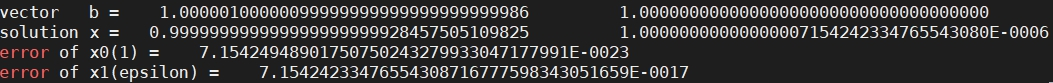
\includegraphics[scale=0.5]{pro1-6.jpg}
        \label{fig1_6} 
    }
    \caption{error of $\epsilon$}
    \label{fig1}
\end{figure}

We change the matrix A to become the equation.4. in the assignment.\\
Noticed that when we declare the variable $\epsilon$, we should make the precision of the variable type become \textbf{real*16}, then we can get a better result of our computer's calculation error.

We know the definition of condition number:
\begin{equation}
    \mbox{cond(A)}=||A||\dot||A^{-1}||
    \label{eq:cond}
\end{equation}

And we get $det(A)=\epsilon^2 \quad det(A^{-1})=1$ , so the condition number of this system is $\epsilon^2$.
For my computer, the value of $\epsilon$ can't show when it's equal to 1e-12.

We are interested in $\sqrt{\epsilon_{mach}}$ , I choose 1e-6 be the value of $\epsilon$, and get the relative error of solution x in component 1 and $\epsilon$(Fig.1(c)).

We know:
\begin{equation}
    \frac{||\triangle x||}{||x||}\leq\mbox{cond(A)}
    \epsilon_{mach}
    \label{eq:error}
\end{equation}

but here the relative error about $\epsilon$ is not obey Eq.\ref{eq:error}. I guess the max $\epsilon_{mach}$ is not equal value 1e-12 (maybe 5e-11...), so my computer can't get good result.\\ \\
% %-------------------------------
\underline{\textbf{Q2 : Cholesky factorization.\\}}

In Fig.2(a)., the pseudo code supplied by the lecture is translated into the fortran code. Noticed that the output variable L don't need to be assigned at the second do loop, because it doesn't finish the process yet when program go to the second loop, the first loop or the moment when we calculate k,k position on the matrix will then get the output result of Cholesky factorization.\\

% %-------------------------------
\begin{figure}[h]
    \centering
    \subfigure[Modification of linalg.f90]{
        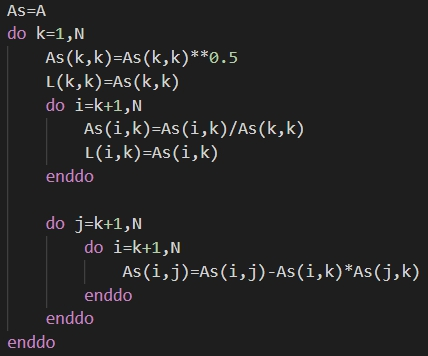
\includegraphics[scale=0.5]{pro2_a.jpg}
        \label{fig2_a}
    }
    \subfigure[the result of writing assignment problem 4]{
        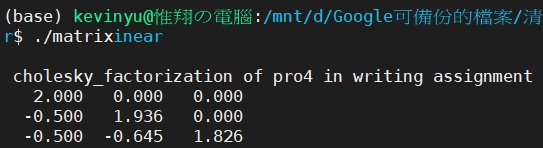
\includegraphics[scale=0.5]{pro2_b.jpg}
        \label{fig2_b} 
    }
    \caption{Cholesky factorization exercise}
    \label{fig2}
\end{figure}
% %-------------------------------
The test of my program is showed in Fig.2(b). The output is the same as the result we get in the written assignments problem 4.\\ \\
%---------------------------------
\underline{\textbf{Q3 : Banded matrix.\\}}

The package of \emph{scipy.linalg.solve\_banded} need to change the banded matrix into the diagonal baned form.
The following is the example of transforming a $7\times7$ banded matrix into the diagonal banded form:

\[
{\begin{bmatrix}
9 &-4 & 1 &0 &0 &0 &0\\
-4& 6 &-4 &1 &0 &0 &0\\
 1&-4 & 6 &-4&1 &0 &0\\
 0& 1 &-4 & 6&-4&1 &0\\
 0& 0 &  1&-4& 6&-4&1\\
 0& 0 &  0& 1&-4& 5&-2\\
 0& 0 &  0& 0& 1&-2& 1
\end{bmatrix}}
\Rightarrow
{\begin{bmatrix}
* &* &1 &1 &1 &1\\
* &-4&-4&-4&-4&-2\\
9 & 6& 6& 6& 5&1\\
-4&-4&-4&-4&-2&*\\
1 &1 &1 &1 &* &*
\end{bmatrix}}
\]

In this example, there are 2 nonzero diagonal below and above the main diagonal, so we can set the variables l \& u which package need to 2 (Fig.3(a). \& Fig.3(b).).

And I also decide two methods to assign the diagonal banded form matrix.  Fig.3(a). judge loop number every time to decide whether the variable is need to be assigned.
Fig.3(b). will continue to execute next loop without doing another if-else judgement.

The time consumption of those three method is showed in Fig.\ref{fig3_time}.\\ \\
% %-------------------------------
\begin{figure}[]
    \centering
    \subfigure[Using solve\_banded package-1]{
        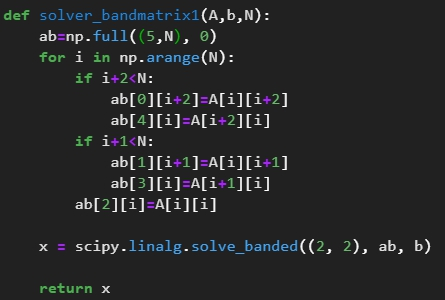
\includegraphics[scale=0.45]{pro3_solver.jpg}
        \label{fig3_sol1}
    }
    \subfigure[Using solve\_banded package-2]{
        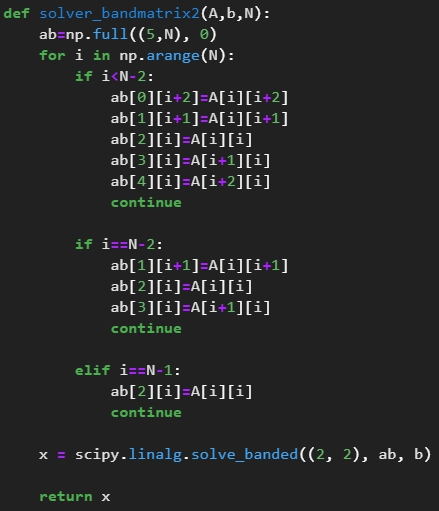
\includegraphics[scale=0.45]{pro3_solver2.jpg}
        \label{fig3_sol2} 
    }
    \subfigure[Using LU decomposition package]{
        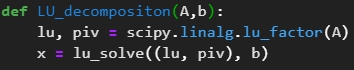
\includegraphics[scale=0.5]{pro3_lu.jpg}
        \label{fig3_lu} 
    }
    \caption{The three method to solve Banded matrix}
    \label{fig3}
\end{figure}
% %-------------------------------
% %-------------------------------
\begin{figure}[]
    \centering 
	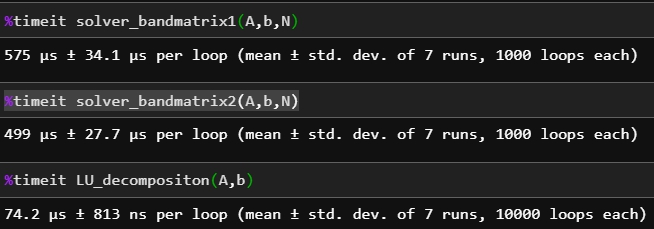
\includegraphics[scale=0.45]{pro3_time.jpg}
	\caption{Time spend by different package in python.} %圖片註解
	\label{fig3_time} %label 用這個就可以引用文章當中
\end{figure}
% %-------------------------------
\underline{\textbf{Q4 : UL factorization.\\}}

\textbf{Verify UL factorization}

In Fig.\ref{fig4_verify}., we first given a matrix $R$, and transpose it into matrix $R^T$, then we inner product these two matrix ,and judge whether it is equal to matrix A in writing assignment problem 4.\\
% %-------------------------------
\begin{figure}[h]
    \centering 
	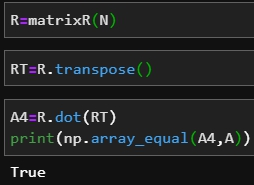
\includegraphics[scale=0.5]{pro4_verify.jpg}
	\caption{Verify UL factorization.} %圖片註解
	\label{fig4_verify} %label 用這個就可以引用文章當中
\end{figure}
% %-------------------------------

\textbf{Solving the system}

In this part, I use the method in problem3.(solver\_bandmatrix2 Fig.2(b).) be the solution of using banded system solver.

And add the comparison: Cholesky factorization was applied by the package in scipy called \emph{linalg.cho\_factor}

The algorithm of my code is used by the code in fortran to transform,
but noticed that: \textbf{the UL factorization has different order to solve compared to LU factorization!}\\
\begin{equation}
    Ax=RR^Tx=ULx=b
\end{equation}
$$Uy=b$$
$$Lx=y$$
The error I derive by the following steps:\\
1.Inner product the matrix A with the solution x to get the experiment b.\\
2.Compare to expected b, get the gap between expected and experiment.\\
3.Finally, sum those error to get the displacement of the calculative error.\\

And we can see that the error generates by UL factorization has even no error.(Fig.\ref{fig4_error}) but spend much more time(Fig.\ref{fig4_time}.) The option of using package or self-coding seem a kind of trade-off.\\

% %-------------------------------
\begin{figure}[h]
    \centering 
	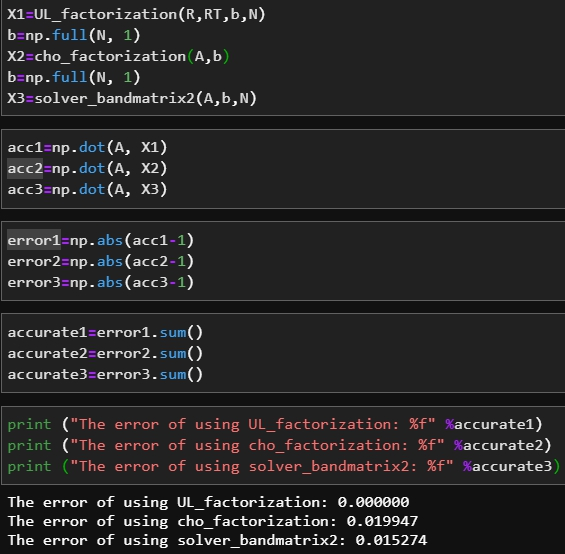
\includegraphics[scale=0.55]{pro4_error.jpg}
	\caption{The accuracy of doing UL factorization by different package.} %圖片註解
	\label{fig4_error} %label 用這個就可以引用文章當中
\end{figure}
% %-------------------------------

% %-------------------------------
\begin{figure}[h]
    \centering 
	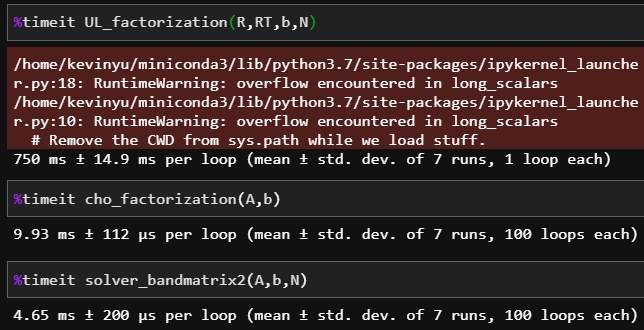
\includegraphics[scale=0.55]{pro4_time.jpg}
	\caption{The time consumption of each algorithm.} %圖片註解
	\label{fig4_time} %label 用這個就可以引用文章當中
\end{figure}
% %-------------------------------

\textbf{Condition number of matrix A}

I use the instruction of numpy called \emph{linalg.cond} to find out the condition number. The output is 1.29e12, it means that this matrix can get pretty accurate solution.(Since larger value of condition number represents nearly singular.)
% %-------------------------------
\begin{figure}[h]
    \centering 
	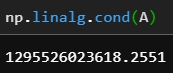
\includegraphics[scale=0.55]{pro4_condition.jpg}
	\caption{condition number of matrix A.} %圖片註解
	\label{fig4_condition} %label 用這個就可以引用文章當中
\end{figure}
% %-------------------------------

\end{document}


% %-------------------------------
% \begin{figure}[h]
%     \centering 
% 	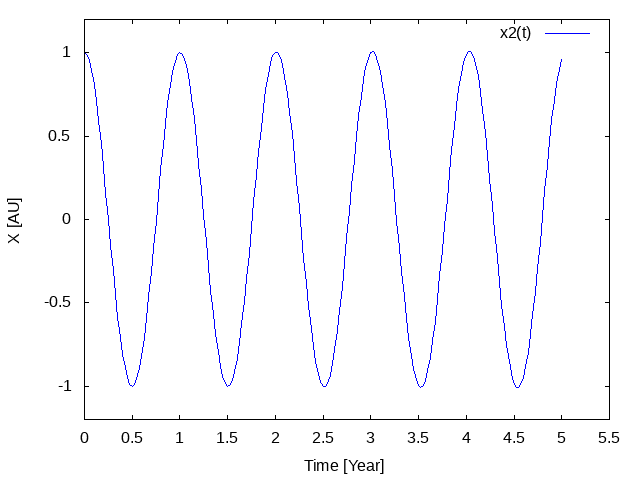
\includegraphics[scale=0.45]{pro1_x2.png}
% 	\caption{The trajectory of $m_1$ $m_2$ (when $m_2$ has a 1.25 factor of velocity).} %圖片註解
% 	\label{fig.pro1} %label 用這個就可以引用文章當中
% \end{figure}
% %-------------------------------

% %-------------------------------
% \begin{figure}[h]
%     \centering
%     \subfigure[dt=0.01yr]{
%         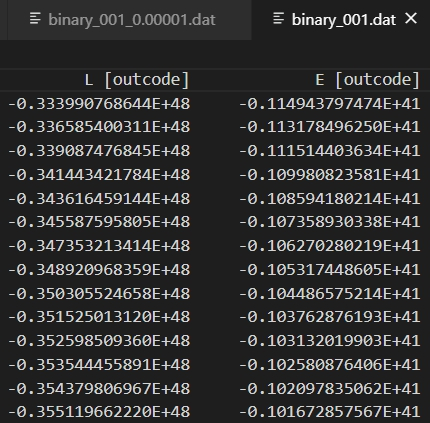
\includegraphics[scale=0.33]{01.jpg}
%         \label{01}
%     }
%     \subfigure[dt=0.001yr]{
%         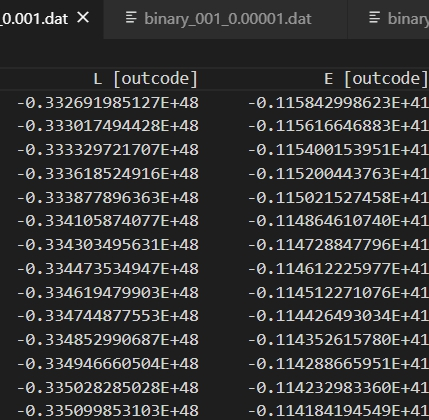
\includegraphics[scale=0.33]{001.jpg}
%         \label{001} 
%     }
%     \subfigure[dt=0.00001yr]{
%         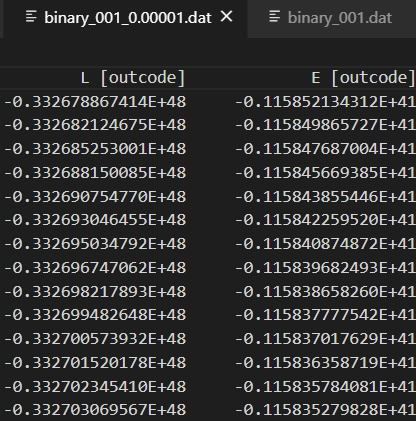
\includegraphics[scale=0.33]{00001.jpg}
%         \label{00001} 
%     }
%     \caption{L \& E in 0.01,0.001,0.00001 time step}
%     \label{fig:2c_dat}
% \end{figure}
% %-------------------------------
